\begin{landscape}
\begin{table}[]
\def\cogimsw{0.19\textwidth}
\centering
\caption{cog preliminary}
\begin{tabular}{@{}lllllll@{}}
\toprule
Render & Input & Segmented & Tagged & Render & Input & Segmented \\ \midrule
\multicolumn{1}{c}{}  & \multicolumn{3}{c}{Office} & \multicolumn{3}{c}{City} \\
\multicolumn{1}{c}{A} &  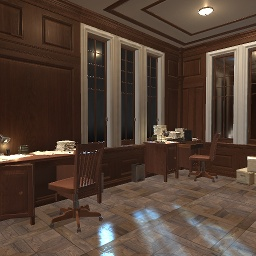
\includegraphics[width=\cogimsw]{Office_A_original} & 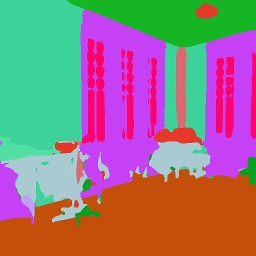
\includegraphics[width=\cogimsw]{Office_A_segmented} & 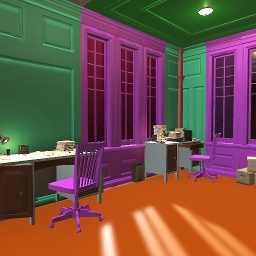
\includegraphics[width=\cogimsw]{Office_A_tagged} & 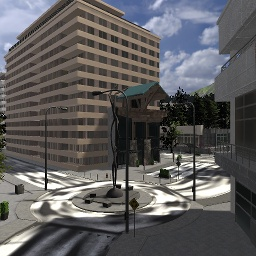
\includegraphics[width=\cogimsw]{City_A_original} & 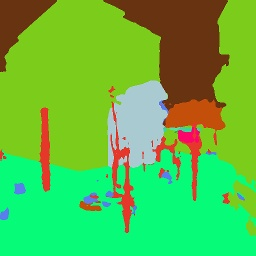
\includegraphics[width=\cogimsw]{City_A_segmented} & 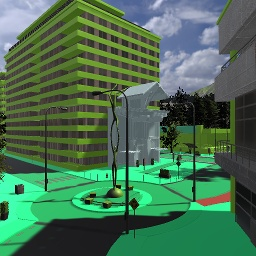
\includegraphics[width=\cogimsw]{City_A_tagged} \\
B & 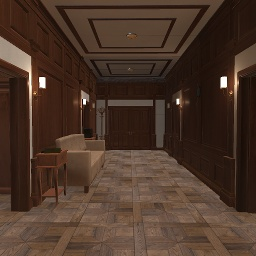
\includegraphics[width=\cogimsw]{Office_B_original} & 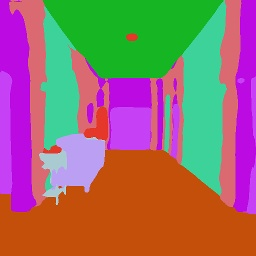
\includegraphics[width=\cogimsw]{Office_B_segmented} & 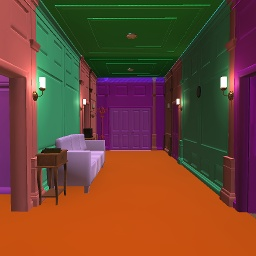
\includegraphics[width=\cogimsw]{Office_B_tagged} & 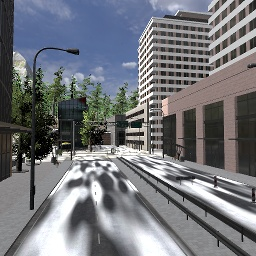
\includegraphics[width=\cogimsw]{City_B_original} & 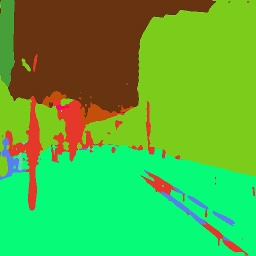
\includegraphics[width=\cogimsw]{City_B_segmented} & 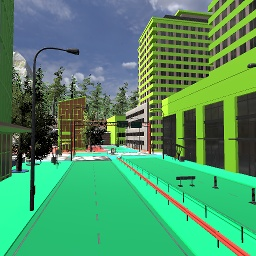
\includegraphics[width=\cogimsw]{City_B_tagged} \\
C & 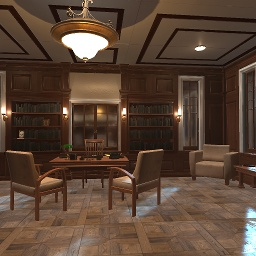
\includegraphics[width=\cogimsw]{Office_C_original} & 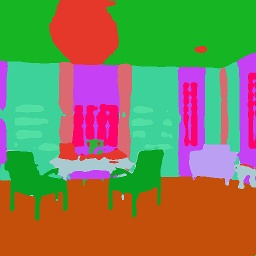
\includegraphics[width=\cogimsw]{Office_C_segmented} & 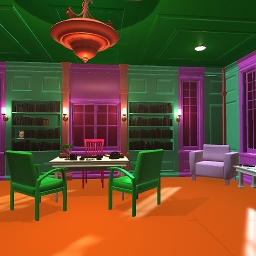
\includegraphics[width=\cogimsw]{Office_C_tagged} & 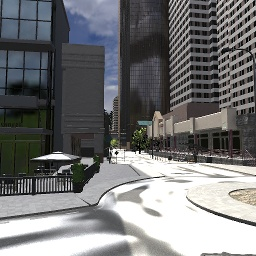
\includegraphics[width=\cogimsw]{City_C_original} & 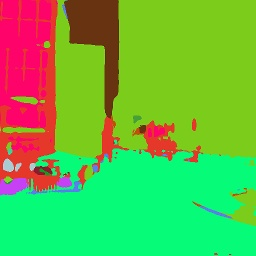
\includegraphics[width=\cogimsw]{City_C_segmented} & 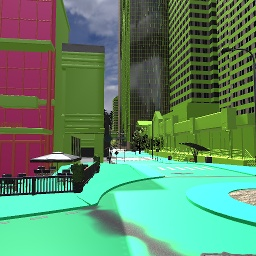
\includegraphics[width=\cogimsw]{City_C_tagged} \\
D & 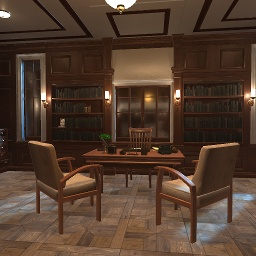
\includegraphics[width=\cogimsw]{Office_D_original} & 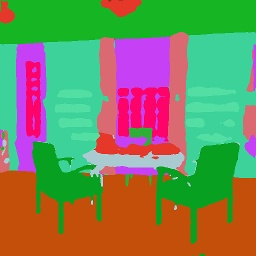
\includegraphics[width=\cogimsw]{Office_D_segmented} & 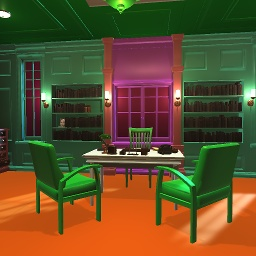
\includegraphics[width=\cogimsw]{Office_D_tagged} & 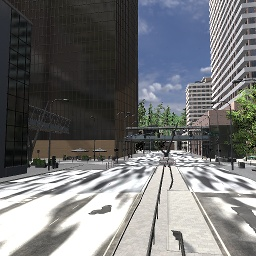
\includegraphics[width=\cogimsw]{City_D_original} & 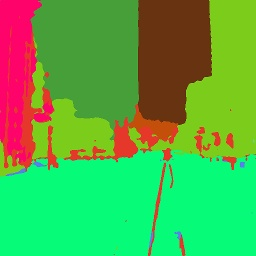
\includegraphics[width=\cogimsw]{City_D_segmented} & 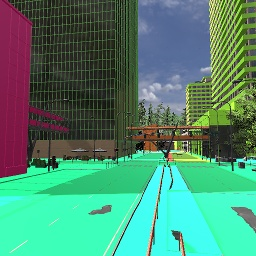
\includegraphics[width=\cogimsw]{City_D_tagged} \\
\multicolumn{1}{l}{legend} & \multicolumn{6}{c}{legend}
\end{tabular}
\label{tab:my-table}
\end{table}
\end{landscape}